%
% teil3.tex -- Beispiel-File für Teil 3
%
% (c) 2020 Prof Dr Andreas Müller, Hochschule Rapperswil
%
\section{Quaternionen}
\rhead{Quaternionen}

Wie die komplexen Zahlen eine Erweiterung der reellen Zahlen sind, sind die Quaternionen eine Erweiterung der komplexen Zahlen für den dreidimensionalen Raum.
Sie haben wie die komplexen Zahlen eine drehstreckende Eigenschaft.
Sie finden beispielsweise in der Computergrafik und Robotik Anwendung.
Die Quaternionen
\begin{align*}
q = w + xi + yj + zk \quad w,x,y,z \in \mathbb{R},\enspace q \in \mathbb{H}
\end{align*}
können dabei eine Drehstreckung mit
\begin{align} \label{QuatRot}
\begin{split} 
v \mapsto v'' = qvq^{-1}
\end{split}
\end{align}
erreichen, falls $q,v,q^{-1} \in \mathbb{H}$ und die Zusammenhänge
\begin{align*}
\operatorname{Re}(q) = \operatorname{Re}(q^{-1})\quad\text{und}\quad \operatorname{Im}(q) = -\operatorname{Im}(q^{-1})
\end{align*}
gelten.
Auffallend ist bei der abbildenden Funktion \eqref{QuatRot} schon die Ähnlichkeit zur Funktion \eqref{rotGA} im Abschnitt~\ref{clifford:section:drehung}.
Man könnte sich nun fragen wieso es drei imaginäre Einheiten $i,j,k$ gibt und nicht zwei, was doch näherliegender wäre.
Der Grund liegt darin, weil es in drei Dimensionen drei Drehachsen gibt, anstatt nur eine.
Wie im Abschnitt~\ref{clifford:section:drehung} beschrieben, können wir auch hier die drei Drehungen durch Linearkombinationen von drei Bivektoren beschreiben.
In der geometrischen Algebra ist es leicht herauszufinden, wie viele Imaginärteile für jede weitere Dimension existieren.
Dabei muss man nur die Anzahl der unabhängigen Bivektoren ermitteln.
In vier Dimensionen würden es beispielsweise durch alle Vektorkombinationen von $\mathbf{e}_1, \mathbf{e}_2,\mathbf{e}_3, \mathbf{e}_4$ insgesamt 8 Bivektoren existieren (Nicht 16, da $\mathbf{e}_{i\!j} = -\mathbf{e}_{ji}$ nicht unabhängig voneinander sind).

Ohne die geometrische Algebra haben wir jetzt aber leider ein kleines Problem.
Für die Darstellung der Quaternionen bräuchten wir insgesamt vier Achsen.
Drei für die imaginären Einheiten und eine für die reelle Einheit.
Ein weiterer Nachteil in visueller Hinsicht entsteht beim Anwenden einer Quaternion auf einen Vektor.
Sie befinden sich nicht im gleichen Raum und müssen zuerst durch
\begin{align}
\mathbf{v} = x\mathbf{\hat{x}} + y\mathbf{\hat{y}} + z \mathbf{\hat{z}} \in \mathbb{R}^3 \enspace\mapsto\enspace v = 0 + xi + yj + zk \in \mathbb{H}
\end{align}
ineinander umgewandelt werden, um damit zu rechnen.

\subsection{Geometrische Algebra}
Die geometrische Algebra kann beide Probleme beheben.
Die Quaternionen können, wie schon im zweidimensionalen Fall durch die Multivektoren gerader Grade $G_3^+(\mathbb{R}) \cong \mathbb{H}$ dargestellt werden.
Da wir uns jetzt aber in $G_3(\mathbb{R})$ befinden haben wir drei Basisvektoren $\mathbf{e}_1, \mathbf{e}_2, \mathbf{e}_3$ und können somit drei Bivektoren $\mathbf{e}_{12}, \mathbf{e}_{23}, \mathbf{e}_{31}$ bilden.
\begin{definition}
	Die Multivektoren mit drehstreckenden Eigenschaften in $G_3(\mathbb{R})$ sind
	\begin{align*}
	\mathbf{q} = w + x\mathbf{e}_{12} + y\mathbf{e}_{23} + z\mathbf{e}_{31} \quad w,x,y,z \in \mathbb{R}\enspace \mathbf{q} \in \mathbb{G}_3^+.
	\end{align*}
\end{definition}

Die Probleme werden dadurch gelöst, dass wir die Bivektoren im Raum nicht durch einzelne Achsen darstellen müssen, sondern sie als eine orientiere Fläche darstellen können.
Anstatt die Vektoren in Quaternionen umzurechnen, können wir jetzt die Vektoren separat im gleichen Raum, wie in Abbildung \ref{BildQuaternionen} gezeigt, darstellen.
\begin{figure}
	\centering
	\includegraphics{papers/clifford/3d/dq.pdf}
	\caption{Darstellung eines Quaternion $\mathbf{q}$ und eines Vektors $\mathbf{v}$ im selben Raum.}
	\label{BildQuaternionen}
\end{figure}

Betrachten wir nun das Produkt
\begin{align*}
\mathbf{qv} &= (w + x\mathbf{e}_{12} + y\mathbf{e}_{23} + z\mathbf{e}_{31})(a\mathbf{e}_1+b\mathbf{e}_2+c\mathbf{e}_3)\\
&= \underbrace{w(a\mathbf{e}_1+b\mathbf{e}_2+c\mathbf{e}_3)}_{\displaystyle{w\mathbf{v}}} + \underbrace{x(-a\mathbf{e}_2+b\mathbf{e}_1}_{\displaystyle{x\mathbf{v}_{\angle 90^\circ, \parallel \mathbf{e}_{12}}}}+c\mathbf{e}_{123}) + \underbrace{y(-b\mathbf{e}_3+c\mathbf{e}_2}_{\displaystyle{y\mathbf{v}_{\angle 90^\circ, \parallel \mathbf{e}_{23}}}}+a\mathbf{e}_{123}) + \underbrace{z(a\mathbf{e}_3-c\mathbf{e}_1}_{\displaystyle{z\mathbf{v}_{\angle 90^\circ, \parallel \mathbf{e}_{31}}}}-b\mathbf{e}_{123}).
\end{align*}
Wie schon im zweidimensionalen Fall \eqref{GAdrehstreck} beschreibt
im dreidimensionalen Fall mit drei Bivektoren jeder Bivektoranteil,
um wie viel der um $90^\circ$ gedrehte, zu der Ebene parallele Teil
des Vektors gestreckt wird.
Dabei dreht jeder Bivektor den Vektor um eine andere Achse und man sieht die drehstreckende Eigenschaft ähnlich zu den komplexen Zahlen.
Der störende Trivektoranteil $(xc+ya+zb)\mathbf{e}_{123}$ bekommt man aber nur weg, indem man, wie in der Drehungsgleichung \eqref{QuatRot}, mit der Inversen Quaternion $\mathbf{q}^{-1}$  multipliziert, wobei die drehgestreckten parallelen Anteile nochmals drehgestreckt werden.
Da nur so der Trivektoranteil wegfällt, sieht man, dass die Drehungsformel der einzige vernünftige Weg ist, mit Quaternionen zu arbeiten.

In der Computergraphik und Robotik macht eine Drehstreckung aber nicht viel Sinn.
Wieso sollte ein Objekt bei einer Drehung zusätzlich noch grösser werden? Darum verwendet man sogenannte Einheitsquaternionen, welche den Betrag $|\mathbf{q}|=1$ haben und somit drehen sie die Objekte bzw.~Vektoren lediglich.
\begin{definition}
	Die Einheitsquaternionen sind definiert als
	\begin{align*}
	\mathbf{q} = \cos(\alpha) + \sin(\alpha)(\tilde{x}\mathbf{e}_{12} + \tilde{y}\mathbf{e}_{23} + \tilde{z}\mathbf{e}_{31})
	\end{align*}
\end{definition}
Zudem setzten wir $\tilde{x}^2+\tilde{y}^2+\tilde{z}^2=1$, damit
\begin{align*}
|\mathbf{q}| = \sqrt{\cos(\alpha)^2 + \sin(\alpha)^2(\tilde{x}^2+\tilde{y}^2+\tilde{z}^2) } = \sqrt{\cos(\alpha)^2 + \sin(\alpha)^2} = 1.
\end{align*}
Der Winkel $\alpha$ beschreibt dabei, wie im Bild \ref{BildQuaternionBeispiel2} gezeigt, den halben Winkel, um welchen der parallelen Anteil $\mathbf{v_{\parallel}}$ des Vektors $\mathbf{v}$ zur kombinierten Bivektorebene $\sin(\alpha)(\tilde{x}\mathbf{e}_{12} + \tilde{y}\mathbf{e}_{23} + \tilde{z}\mathbf{e}_{31})$ gedreht wird.

Um einen Vektor zu drehen, verwendet man die in Abschnitt 18.4 hergeleitete Formel 
\begin{align} \label{QuatRotGA}
\mathbf{v}'' = \mathbf{qvq}^{-1},
\end{align}
wobei wie auch schon bei den Quaternionen gelten muss, dass
\begin{align} \label{GAReIm}
\operatorname{Re}(\mathbf{q}) = \operatorname{Re}(\mathbf{q}^{-1}) \quad\text{und}\quad \operatorname{Im}(\mathbf{q}) = -\operatorname{Im}(\mathbf{q}^{-1}).
\end{align}
Der Grund für die Zusammenhänge \eqref{GAReIm} kann man durch die hergeleitete vereinfachte Drehungsgleichung \eqref{GAvereinfRot} sehen, weil durch den negierten Winkel $\vartheta$ der reelle bzw.~Grad~0-Anteil
\begin{align*}
\operatorname{Re}(e^{-\vartheta \mathbf{e}_{12}}) = \operatorname{Re}(e^{\vartheta \mathbf{e}_{12}})
\end{align*}
und der imaginäre bzw.~Grad~2-Anteil
\begin{align*}
\operatorname{Im}(e^{-\vartheta \mathbf{e}_{12}}) = -\operatorname{Im}(e^{\vartheta \mathbf{e}_{12}})
\end{align*}
ist.
Durch die geometrische Algebra sieht man nun, wieso es wichtig ist, bei Quaternionen für eine reine Drehstreckung mit $\mathbf{q}$ und $\mathbf{q}^{-1}$ beidseitig zu multiplizieren, sonst werden die senkrechten Anteile zu den Bivektorebenen ebenfalls beeinflusst, wie man im Abschnitt~\ref{clifford:section:drehung} bei der Formel \eqref{RotAufPerpPar} sehen kann.
\begin{beispiel}
	Eine Drehung eines Vektors $\mathbf{v}= 1\mathbf{e}_2$ um $90^\circ$ um die $\mathbf{e}_1$-Achse und danach $90^\circ$ um die $\mathbf{e}_2$-Achse.
Dafür nehmen wir zuerst die Einheitsquaternion 
	\[
	\begin{aligned}
	\mathbf{q}_{23}
	&=
	\cos(\pi/4) + \sin(\pi/4)(1\mathbf{e}_{23}) = e^{(\pi/4)\mathbf{e}_{23}}
	&
	&=
	\textstyle{\frac{\sqrt{2}}{2}}(1 + \mathbf{e}_{23})
	\\
	\mathbf{q}_{23}^{-1}
	&
	&
	&= \textstyle{\frac{\sqrt{2}}{2}} (1- \mathbf{e}_{23})
	\end{aligned}
	\]
welche um die $\mathbf{e}_{2}$-$\mathbf{e}_{3}$-Ebene um $90^\circ$ dreht und danach die Einheitsquaternion 
	\[
	\begin{aligned}
	\mathbf{q}_{31}
	&=
	\cos(\pi/4) + \sin(\pi/4)(1\mathbf{e}_{31})
	=
	e^{(\pi/4)\mathbf{e}_{31}}
	&
	&=
	\textstyle{\frac{\sqrt{2}}{2}}(1 + \mathbf{e}_{31})
	\\
	\mathbf{q}_{31}^{-1}
	&
	&
	&= \textstyle{\frac{\sqrt{2}}{2}}(1 - \mathbf{e}_{31}),
	\end{aligned}
	\]
	welche um die $\mathbf{e}_{3}$-$\mathbf{e}_{1}$-Ebene  um $90^\circ$ dreht.
Um die vollständige Drehung zu beschreiben, können die Einheitsquaternionen multipliziert werden, wobei die Reihenfolge der Ausführung beachtet werden muss.
Somit ist
\begin{align}
\label{FormelBeispielQuaternion}
\mathbf{q}
&=
\mathbf{q}_{31}\mathbf{q}_{23}
=
\textstyle{\frac{\sqrt{2}}{2}}(1 + \mathbf{e}_{31})\textstyle{\frac{\sqrt{2}}{2}}(1 + \mathbf{e}_{23})
&
&=
\textstyle{\frac{1}{2}}(1 + \mathbf{e}_{31} + \mathbf{e}_{23} + \mathbf{e}_{12})
\\
\mathbf{q}^{-1}
&=
\mathbf{q}_{23}^{-1}\mathbf{q}_{31}^{-1}
=
\textstyle{\frac{\sqrt{2}}{2}} (1- \mathbf{e}_{23})\textstyle{\frac{\sqrt{2}}{2}}(1 -\mathbf{e}_{31})
&
&=
\textstyle{\frac{1}{2}}(1 - \mathbf{e}_{31} - \mathbf{e}_{23} - \mathbf{e}_{12}).
\notag
\end{align}
	Wenn wir nun die Quaternion $\mathbf{q}$ auf den Vektor $\mathbf{v}$ anwenden, erhalten wir
	\begin{align*}
	\mathbf{v}'' = \mathbf{qvq}^{-1} &= \textstyle{\frac{1}{2}}(1 + \mathbf{e}_{31} +  \mathbf{e}_{23} +  \mathbf{e}_{12})(1\mathbf{e}_2)\textstyle{\frac{1}{2}}(1 - \mathbf{e}_{31} -  \mathbf{e}_{23} -  \mathbf{e}_{12})\\ 
	&= \textstyle{\frac{1}{4}}(\mathbf{e}_2 +  \mathbf{e}_{123} -  \mathbf{e}_3 +  \mathbf{e}_1)(1 - \mathbf{e}_{31} -  \mathbf{e}_{23} -  \mathbf{e}_{12})\\
	&= (\textstyle{\frac{1}{4}} + \textstyle{\frac{1}{4}} + \textstyle{\frac{1}{4}} + \textstyle{\frac{1}{4}})\mathbf{e}_1 + (\textstyle{\frac{1}{4}} + \textstyle{\frac{1}{4}} - \textstyle{\frac{1}{4}} - \textstyle{\frac{1}{4}})\mathbf{e}_2 +\\ &\qquad(-\textstyle{\frac{1}{4}} + \textstyle{\frac{1}{4}} - \textstyle{\frac{1}{4}} + \textstyle{\frac{1}{4}})\mathbf{e}_3 + (\textstyle{\frac{1}{4}} - \textstyle{\frac{1}{4}} - \textstyle{\frac{1}{4}} + \textstyle{\frac{1}{4}})\mathbf{e}_{123}\\
	&= 1e_1. 
	\end{align*}
	Anders betrachtet könnte man von der Formel \eqref{FormelBeispielQuaternion} sehen, dass der Drehwinkel
	\begin{align*}
	\alpha = \arccos(w) = \arccos(\textstyle{\frac{1}{2}}) = 60^\circ
	\end{align*}
	und die Ebene der kombinierten Bivektoren wie in Abbildung \ref{BildQuaternionBeispiel2} aussieht.
	Somit kann man sich ebenfalls vorstellen, wie der parallele Anteil zur Ebene insgesamt um 120° gedreht wird, während der senkrechte Anteil unverändert bleibt.
\end{beispiel}

\begin{figure}
	\centering
	\includegraphics{papers/clifford/3d/qq.pdf}
	
	\caption{Beispiel für Drehung um $90^\circ$ je um die $\mathbf{e}_1$- und $\mathbf{e}_2$-Achse.}
	\label{BildQuaternionBeispiel}
\end{figure}

\begin{figure}
	\centering
	\includegraphics{papers/clifford/3d/drehung.pdf}
	\caption{Beim Beispiel wird der parallele Anteil um 120° gedreht während der senkrechte Anteil zur kombinierten Ebene (Bivektoraddition) gleich bleibt.}
	\label{BildQuaternionBeispiel2}
\end{figure}

\subsection{Interpolation}
\index{Interpolation}%
In der Computergrafik wird Interpolation verwendet, um eine flüssige Drehbewegung zu erreichen.
Dabei wird die ganze gewünschte Drehbewegungen des Objektes in kleinere Drehbewegungen aufgeteilt, wobei diese zeitlich nacheinander auf das Objekt angewendet werden.
Als Vergleich könnte man sagen, dass ein Film auch nur Bilder sind, welche zeitlich nacheinander gezeigt werden.
Man kann dabei mit zwei verschiedenen Systemen arbeiten.
\begin{itemize}
	\item Mit den eulerschen Winkeln, welche für die meisten zwar intuitiver sind, aber dafür Nachteile haben, worauf
in diesem Abschnitt eingegangen werden soll.
Dabei kann eine ganze Drehbewegung $\mathbf{v}'' = R\mathbf{v}$ durch die Drehmatrix
	\begin{align} \label{GADrehmatrix}
	R = 
	\underbrace{
		\begin{pmatrix} 
		\cos(\gamma) & -\sin(\gamma) & 0\\ \sin(\gamma) & \cos(\gamma) & 0 \\ 0 & 0 & 1 
		\end{pmatrix}
	}_{\displaystyle{R_z(\gamma)}}
	\underbrace{
		\begin{pmatrix}
		\cos(\beta) &  0 & \sin(\beta)\\ 0 & 1 & 0 \\ -\sin(\beta) & 0 & \cos(\beta)
		\end{pmatrix}
	}_{\displaystyle{R_y(\beta)}}
	\underbrace{
		\begin{pmatrix} 
		1 & 0 & 0 \\ 0 & \cos(\alpha) & -\sin(\alpha)\\ 0 & \sin(\alpha) & \cos(\alpha)
		\end{pmatrix}
	}_{\displaystyle{R_x(\alpha)}}
	\end{align}
	dargestellt werden.
Wichtig dabei zu sehen ist, dass die Drehbewegungen durch die einzelnen Matrizen nacheinander ausgeführt werden.
Das bedeutet, wenn man die Reihenfolge vertauscht, bekommt man eine völlig andere Drehung.
Man kann die Auswirkungen der Reihenfolge gut bei einem Gimbal im Bild \ref{BildReihenfolgeGimbal} sehen.
Die Matrix ganz links in der Gleichung~\eqref{GADrehmatrix} ist die, welche als letztes angewendet wird.
Somit bildet sie die Drehung des äusseren Rings, welche auch die zwei inneren Ringe und das Objekt mitdreht.
Die Matrix ganz rechts hingegen bildet nur die Drehung des inneren Rings, welche nur das Objekt mitdreht.
Man kann dabei erkennen, dass das Vorgehen zwar sehr intuitiv ist, aber es kompliziert sein kann, eine gewünschte Drehbewegung auszuführen, da sich beim Drehen der äusseren Achse, sich auch die inneren drehen.
Das bedeutet, wenn man sich eine Drehbewegung um die anfängliche $x$-Achse mit $R_x(\alpha_2)$ wünscht, und vorher eine beliebige Drehung $R = R_z(\gamma_1) R_y(\beta_1) R_x(\alpha_1)$ ausgeführt hat, bekommt man nicht das richtige Ergebnis, da die anfängliche $x$-Achse durch die Drehmatrizen $R_z(\gamma_1)$ und $R_y(\beta_1)$ zu einer neuen, lokalen $x$-Achse wurde.

	\item Mit den Quaternionen, welche die besondere Eigenschaft haben, dass eine Drehung immer um die globale Achse ausgeführt wird, egal in welcher Drehungsposition sich das Objekt befindet.
\end{itemize}
Für Spielentwickler ist es darum meist sinnvoller Quaternionen für Drehbewegungen anzuwenden, als sich mit komplizierten Berechnungen mit Eulerschen Winkeln herumzuschlagen.

\begin{figure}
	\centering
	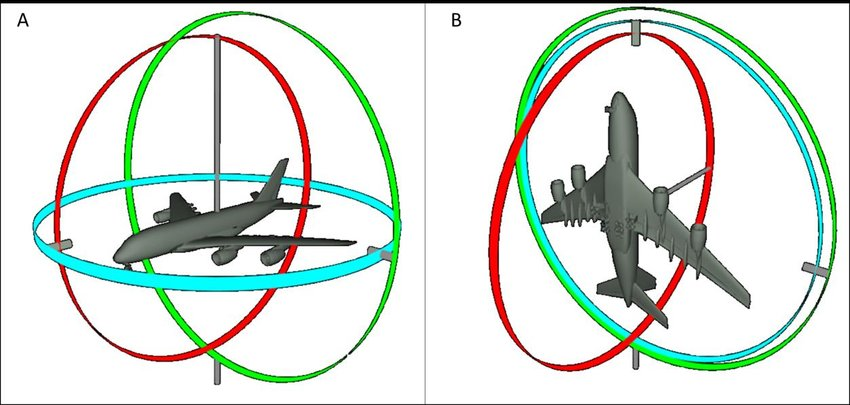
\includegraphics[width=10cm]{papers/clifford/Bilder/ReihenfolgeGimbal.png}
	\caption{Das Gimbal Lock tritt ein, wenn zwei Drehachsen in der gleichen Ebene liegen. Dies ist im rechten Bild bei der grünen und blauen Achse der Fall. Der rote Kreis würde sich an der oberen Halterung genau in die gleiche Richtung drehen, wie der grüne Kreis an der unteren Halterung. Man verliert somit eine Drehrichtung.}
	\label{BildReihenfolgeGimbal}
\end{figure}

\subsection{Gimbal-Lock}
Ein weiterer Nachteil der Eulerschen Winkel ist das Gimbal-Lock.
Es entsteht dann, wenn zwei Ringe Deckungsgleich übereinander gedreht werden, wie man im Bild \eqref{BildReihenfolgeGimbal} sieht.
Dabei verliert das Gimbal eine Drehrichtung, da der äussere und innere Ring nun die gleiche Drehrichtung besitzen.
Dies kann beispielsweise Probleme bei Spielen bei der Berechnung der Interpolation führen.
Man hat dies bei älteren Spielen wie im Bild \ref{BildGimbalLock} dann gesehen, wenn plötzlich Gliedmassen bei den Spielermodellen in unnatürliche Richtungen gesprungen sind.

\begin{figure}
	\centering
	\includegraphics[width=10cm]{papers/clifford/Bilder/GimbalLock.png}
	\caption{Interpolationsfehler durch Gimbal-Lock}
	\label{BildGimbalLock}
\end{figure}
